%-------------------------------------------------------------------------------
% LATEX TEMPLATE ARTIKEL
%-------------------------------------------------------------------------------
% Dit template is voor gebruik door studenten van de de bacheloropleiding 
% Informatica van de Universiteit van Amsterdam.
% Voor informatie over schrijfvaardigheden, zie 
%                               https://practicumav.nl/schrijven/index.html
%
%-------------------------------------------------------------------------------
%	PACKAGES EN DOCUMENT CONFIGURATIE
%-------------------------------------------------------------------------------

\documentclass{uva-inf-article}
\usepackage[english]{babel}
\usepackage{tikz}
\usepackage{pdflscape}
\usepackage{todonotes}
\usepackage{listings}
\lstset{
basicstyle=\small\ttfamily,
columns=flexible,
breaklines=true
}

\usepackage[style=authoryear-comp]{biblatex}
\addbibresource{references.bib}

%-------------------------------------------------------------------------------
%	GEGEVENS VOOR IN DE TITEL, HEADER EN FOOTER
%-------------------------------------------------------------------------------

% Geef je artikel een logische titel die de inhoud dekt.
\title{Unreal Engine Documentation}

% Vul de naam van de opdracht in zoals gegeven door de docent en het type 
% opdracht, bijvoorbeeld 'technisch rapport' of 'essay'.
% \assignment{}
% \assignmenttype{}

% Vul de volledige namen van alle auteurs in en de corresponderende UvAnetID's.
\authors{Jari Andersen}
% \uvanetids{}

% Vul de naam van je tutor, begeleider (mentor), of docent / vakcoördinator in.
% Vermeld in ieder geval de naam van diegene die het artikel nakijkt!
% \tutor{}
% \mentor{}
% \docent{}

% Vul hier de naam van je tutorgroep, werkgroep, of practicumgroep in.
% \group{SignLab, VisualisationLab}

% Vul de naam van de cursus in en de cursuscode, te vinden op o.a. DataNose.
% \course{}
% \courseid{}

% Dit is de datum die op het document komt te staan. Standaard is dat vandaag.
\date{\today}

%-------------------------------------------------------------------------------
%	VOORPAGINA 
%-------------------------------------------------------------------------------

\begin{document}
\maketitle

%-------------------------------------------------------------------------------
%	INHOUDSOPGAVE EN ABSTRACT
%-------------------------------------------------------------------------------
% Niet toevoegen bij een kort artikel, zeg minder dan 10 pagina's!

%TC:ignore
\tableofcontents
%\begin{abstract}
%\end{abstract}
%TC:endignore
\newpage
%-------------------------------------------------------------------------------
%	INHOUD
%-------------------------------------------------------------------------------
% Hanteer bij benadering IMRAD: Introduction, Method, Results, Discussion.
\section{Introduction}
Welcome to this comprehensive documentation compiled during the development journey in Unreal Engine. Throughout this document, you'll find information encompassing various aspects of development, ranging from the utilization of C++, Blueprints, and Python to defining structs for data tables. We'll also explore best practices and strategies for implementing Git, ensuring efficient collaboration and version control. Mostly, we'll touch upon bugs that we've encountered and hopefully fixed. This documentation aims to provide valuable insights and practical guidance for Unreal Engine projects.

\subsection{Live Link}
For the Live Link Pipeline documentation, go to the Unreal Live Link Pipeline documentation repository (\url{https://github.com/J-Andersen-UvA/LiveLinkPipeline-UnrealEngine}).

% \begin{landscape}
% \vspace*{\fill}
% \begin{figure}[hbt!]
%     \centering
%     \includegraphics[width=1.5\textheight]{imgs/pipeline16-2-24.png}
%     \caption{Current Live Link Pipeline. Three streams into Unreal Engine}
%     \label{fig:pipeline}
% \end{figure}
% \vspace*{\fill}
% \end{landscape}

\section{Compiling and building C++ projects}\label{CompilingAndBuilding}
When it comes to building the C++ files in Unreal we either use the IDE or Unreal Engine. Unreal Engine's compilation system comes with a functionality called Live Coding. Live coding with "hot reloading" allows developers to make changes to their C++ code while the game is running and see the changes reflected in real-time without the need to restart the game or editor. For our purposes (and because it causes many bugs), we disable the Live Coding option (see Figure \ref{fig:liveCoding} on where to disable this, and Section \ref{datatableBug} on an example bug caused by Live Coding).
\begin{figure}[hbt!]
    \centering
    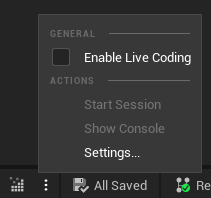
\includegraphics{imgs/livecoding.png}
    \caption{Where to disable Live Coding}
    \label{fig:liveCoding}
\end{figure}

Now we can compile in Unreal Engine or in an IDE like Visual Studio. Figure \ref{fig:vstudio} shows where to build using Visual Studio. Do make sure to follow the instructions in the following link to setup the Build tool first: \url{https://docs.unrealengine.com/4.27/en-US/ProductionPipelines/DevelopmentSetup/BuildingUnrealEngine/}. As for Unreal Engine, use the button showed in Figure \ref{fig:liveCoding}.

\begin{figure}[hbt!]
    \centering
    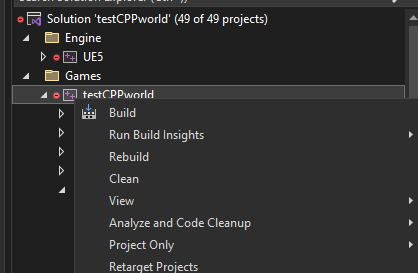
\includegraphics{imgs/buildingInVStudio.png}
    \caption{Where to build using Visual Studio}
    \label{fig:vstudio}
\end{figure}
\section{Git Version control}
We use Git for Unreal Engine to efficiently manage project versions, and to enable collaboration among team members. Git allows us to track changes to code, blueprints, and assets. By utilizing Git, Unreal Engine developers can maintain organized workflows, iterate rapidly, and coordinate effectively on complex projects.

\subsection{How to install and use Git for Unreal Engine}
Adding project to a blank repository Git:
\begin{enumerate}
    \item In the bottom right of a level screen in Unreal Engine, click revision control.
    \item Select connect to revision control.
    \item After selecting Git, add the url of your repository and initialize.
\end{enumerate}

Now you can use the same revision control button to add changes, write commits and view changes. You do however, need to push the commits by hand.
Note that sometimes some files aren't added to the Git, you'll have to fix that by adding them by hand.

\subsection{Local Plugins}
In Unreal Engine, third-party plugins play a significant role in extending functionality and enhancing project capabilities. However, unlike native plugins bundled within the Engine plugins folder, third-party plugins must be added to the project's root plugins folder due to the engine's architecture.

When we add plugins locally however, the plugins will be pushed with the rest of the project. This can cause bugs later on (see Section \ref{cppThirdPartyPluginsBug}). Especially for cloning the repository on a new machine this causes issues (follow Section \ref{cloning} for best practices on cloning a repository).

\subsection{Cloning}\label{cloning}
When cloning a repository everything usually works well. There are cases however, when cloning a repository breaks the build (for example \ref{cppThirdPartyPluginsBug}).
If we open a new project that is broken, Unreal Engine will prompt us if he can rebuild it. This works sometimes, but in cases where a local plugin prevents us to build we can do a simple trick:
\begin{itemize}
    \item Move the local plugin out of the project.
    \item Rebuild in your IDE.
    \item Open the project.
    \item Put the plugin back and rebuild.
\end{itemize}

\section{Thoughts on using C++, Python, and Blueprints}
After fighting a bit in Unreal with Python, C++, and Blueprints, we have formed thoughts on how to use and when to apply these tools. For example, C++ has nice integration with Blueprints, and it seems to be the normal way of coding in Unreal Engine. We have seen other code bases that integrate both. Therefore, we will not migrate everything to C++, but we will integrate C++ into our workflow for Unreal Engine. We can say similar things about Python. It has its own strengths, especially when coupling it with our other code that already use sockets to communicate. It is however, rather slow if we try to insert functions on every tick. With these thoughts and experiences, we decided that we will need to make careful considerations before picking our "tool" to tackle a problem.

\section{Bugs and fixes}
In the "Bugs and Fixes" section, we address challenges we encountered in Unreal Engine development hopefully along with their solutions.

\subsection{C++ projects and third party plugins}\label{cppThirdPartyPluginsBug}
Using third party plugins enables us to focus on our own development. It does come with its own challenges, however. One of which we encountered when migrating to C++ based projects. When trying to compile a project that uses third party plugins from the Engine folder that are not in the marketplace we get reference errors, example:
\begin{lstlisting}
Expecting to find a type to be declared in a module rules named 'MoCapProLiveLink' in UE5Rules, Version=0.0.0.0, Culture=neutral, PublicKeyToken=null.  This type must derive from the 'ModuleRules' type defined by Unreal Build Tool.
\end{lstlisting}
Most tips on the internet tell us to move the plugins to a project root folder called Plugins. This works, but it causes issues with the Git integration (see Section \ref{cloning} on how to fix this). One might think that we can add the module names to the build file, but in our case that did not help solve the issue.

\subsection{Datatable bug}\label{datatableBug}
Previously, we stored ``blendshape source" data, ``blendshape target" data, ``weight" data, and ``multiple blendshapes to drive" data separately within maps and arrays in blueprints. This is very redundant so we decided to move these structures to be encapsulated in a single C++ Struct. After coding this in C++ and creating a datatable out of this in Unreal Engine, we populated it with data (an example of a single entry can be seen in Figure \ref{fig:blendshapeStructExample}).

\begin{figure}[hbt!]
    \centering
    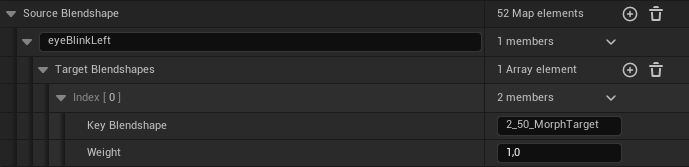
\includegraphics[width=\textwidth]{imgs/singleBlendshapeData.png}
    \caption{An example source blendshape that drives a single target blendshape with a weight of 1.}
    \label{fig:blendshapeStructExample}
\end{figure}

This worked very well until we closed the editor, re-opened it and tried to view the datatable again. We get prompted by Unreal with an Error message. Pressing "Yes" at error message will open the asset without any of the struct information. Where did our data go? After a lot of fighting, we broke the entire project again and we had to rebuild through our IDE. Somehow that fixed the issue for the datatable as wel. Later into development the table was not useable in a blueprint, however. After further inspection we noticed that the ``RowStruct" of the datatable changed to something prepended with ``LIVECODE". Therefore we concluded that the entire problem was caused by the hotloading functionality of Unreal's compilation system. Disabling this functionality fixed the problem (more on best practices for compiling in Section \ref{CompilingAndBuilding}).

\subsection{Exporting/importing Datatables}
When exporting a datatable, you might be tempted to export it the same way you would export any other asset. That doesn't work however. Simply export it as csv or json in order to import it in a new project. In the new project, create a new datatable, open it, and use the reimport button to import the csv or json.

%-------------------------------------------------------------------------------
%	REFERENTIES
%-------------------------------------------------------------------------------

\printbibliography

%-------------------------------------------------------------------------------
%	BIJLAGEN 
%-------------------------------------------------------------------------------

%TC:ignore
% \appendix 
% \section{Bijlage {\LaTeX} code}
% Bijgevoegd zijn de \textattachfile{main.tex}{code} en 
% \textattachfile{references.bib}{bibliografie}.
%TC:endignore

%-------------------------------------------------------------------------------
\end{document}